\chapter{Конструкторская часть}

На основе формализованных требований к базе данных и выбора её типа может быть выполнено её проектирование.
В данном разделе будут спроектированы сущности базы данных, её ролевая модель а также архитектура погодного приложения.

\section{Диаграмма сущность-связь}
На рисунках~\ref{fig:er-barker}--\ref{fig:er-chen} представлена диаграмма сущность-связь для разрабатываемой базы данных в нотации Баркера.
Каждая отдельная сущность соответствует ровно одной таблице в реляционной базе данных.
\begin{figure}[H]
	\centering
	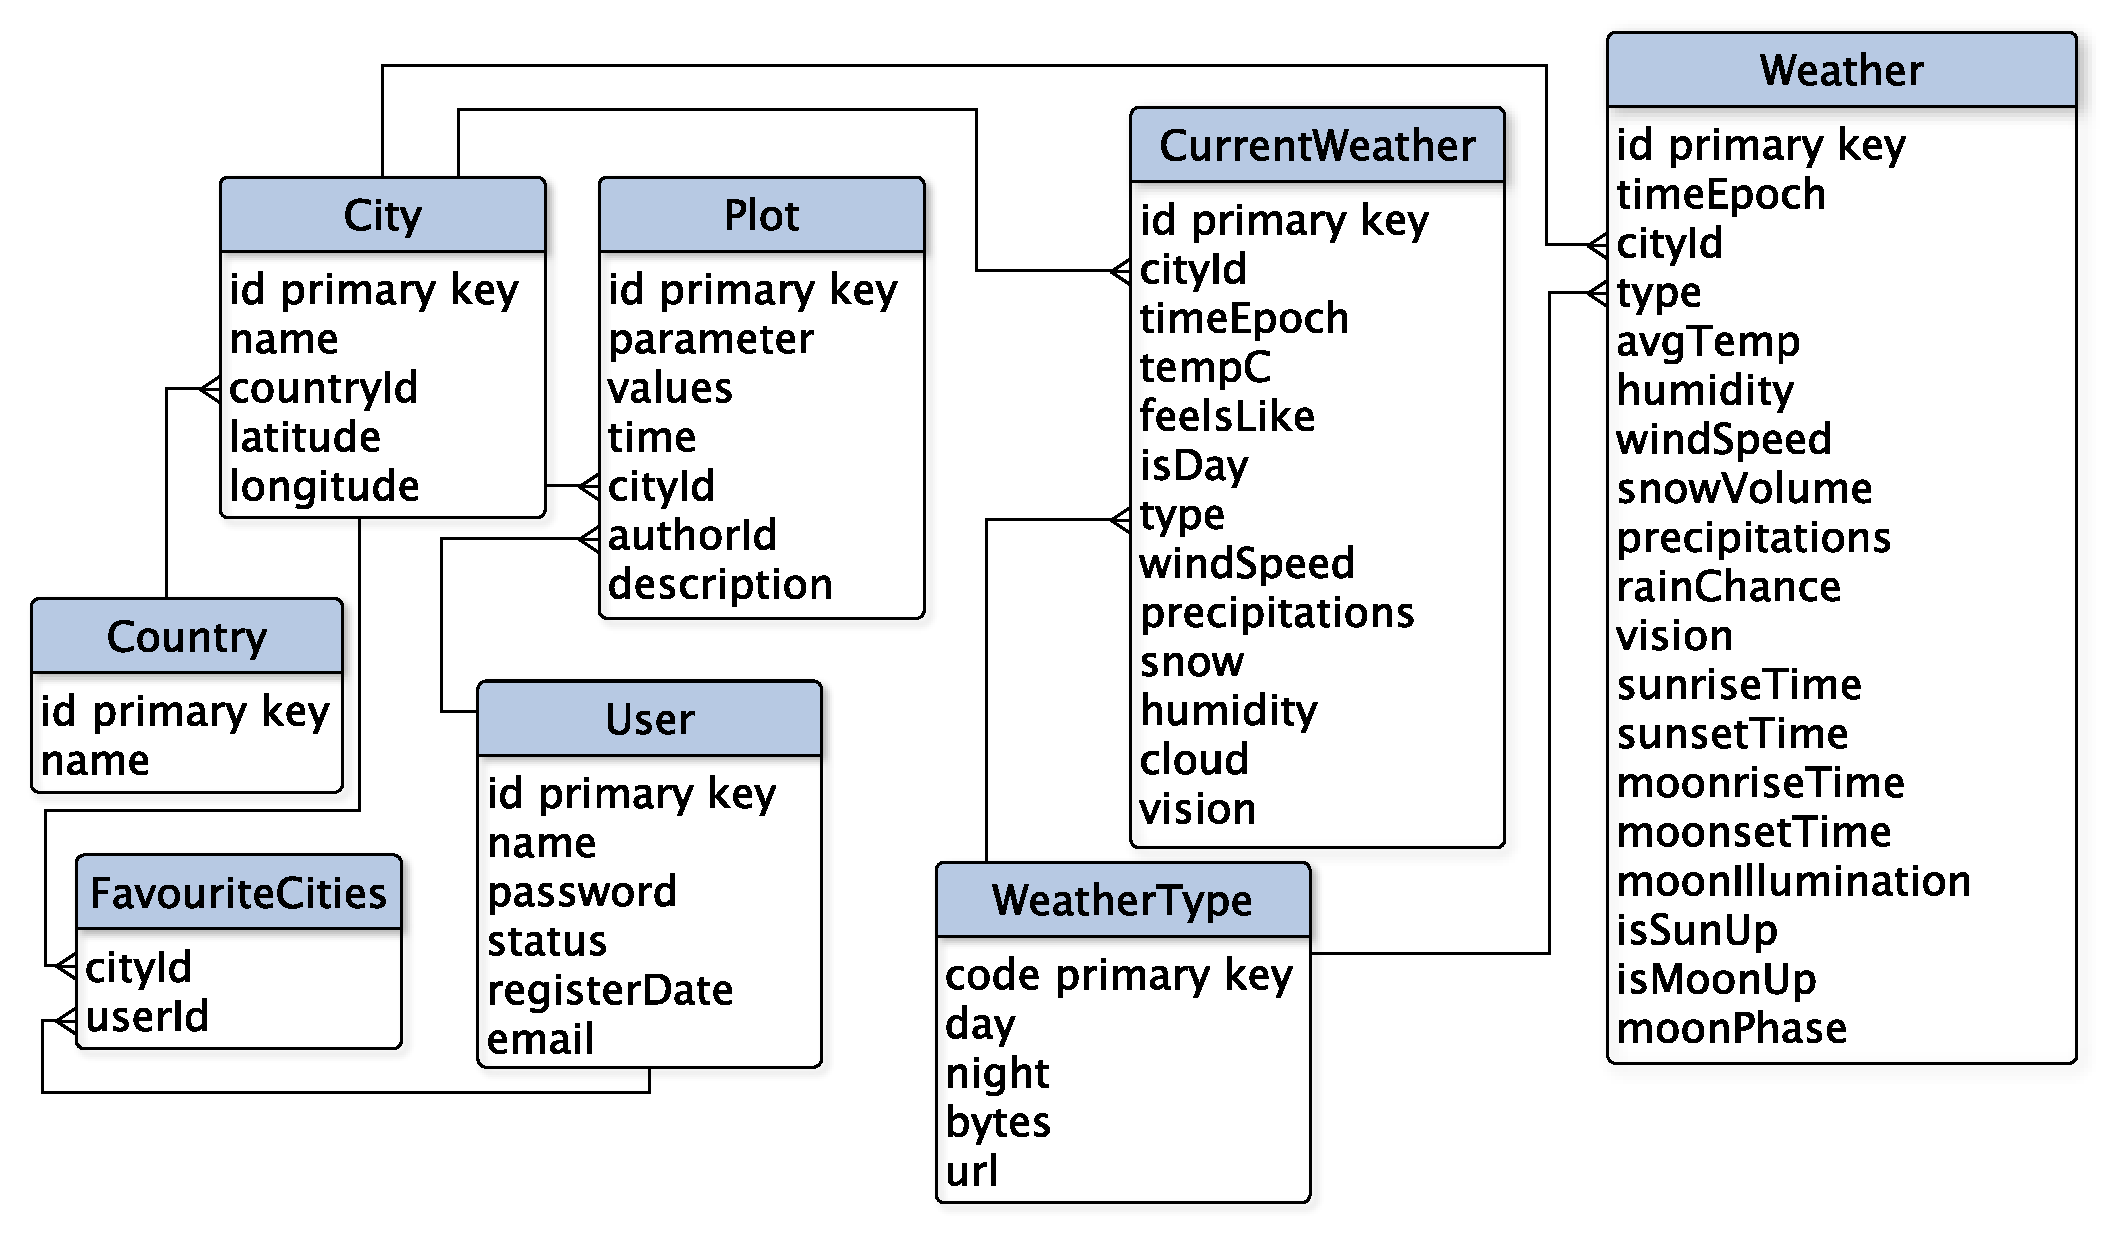
\includegraphics[width=\textwidth]{tools/img/er-barker.pdf}
	\caption{
        Диаграмма сущность-связь разрабатываемой базы данных в нотации Баркера
    }
	\label{fig:er-barker}
\end{figure}

\section{Проектирование сущностей базы данных}

На этапе анализа определены сущности, которые будут храниться в базе данных.
Необходимо определить тип данных, которым представляется каждый их атрибут, а также атрибуты для идентификации и связи с другими сущностями.
Один из атрибутов каждой сущности -- её идентификатор.
Он представляет собой целое число.
Далее рассмотрена каждая сущность в отдельности.

\subsection*{Погода}
Погода связана с городом, который является отдельной сущностью.
Тогда она должна хранить его идентификатор как внешний ключ.
Другой внешний ключ -- идентификатор типа погоды.
Остальные параметры погоды хранятся как целые или вещественные числа или как строки.
Таблица~\ref{table:weather_attr} отображает, какие атрибуты имеют сущности суточной и часовой погоды, а также типы этих атрибутов.

\begin{table}[h!]
    \centering
    \begin{tabular}{ |c|c|c|c| }
        \hline
        \multicolumn{2}{|c|}{Атрибут} & \multicolumn{2}{|c|}{Погода}  \\
        \hline
            \textbf{Назначение} & \textbf{Тип} & \textbf{Суточная} & \textbf{Часовая} \\
        \hline
            id & целое число & + & + \\
        \hline
            время & целое число & + & + \\
        \hline
            id города & целое число & + & + \\
        \hline
            тип & целое число & + & + \\
        \hline
            температура & вещественное число & + & + \\
        \hline
            влажность & целое число & + & + \\
        \hline
            скорость ветра & целое число & + & + \\
        \hline
             снег & целое число & + & + \\
        \hline
             осадки & целое число & + & + \\
        \hline
             видимость & вещественное число & + & + \\
        \hline
             облачность & целое число & + & + \\
        \hline
             вероятность дождя & целое число & + & - \\
        \hline
             восход солнца & целое число & + & - \\
        \hline
             восход луны & целое число & + & - \\
        \hline
             закат солнца & целое число & + & - \\
        \hline
             закат луны & целое число & + & - \\
        \hline
             освещённость луны & целое число & + & - \\
        \hline
             фаза луны & строка & + & - \\
        \hline
             наличие луны & логический & + & - \\
        \hline
            день или ночь & логический & - & - \\
        \hline
            ощущаемая температура & целое число & - & + \\
        \hline
            
    \end{tabular}
    \caption{\centering Атрибуты погоды}
    \label{table:weather_attr}
\end{table}

\subsection*{Город и страна}
Далее рассматривается сущность города.
Идентификатор страны является внешним ключом для города.
Поэтому ситуация, когда два города из одной страны хранят её название по-разному, невозможна.
В таблице~\ref{table:city_attr} представлены атрибуты страны и города.
\begin{table}[h!]
    \centering
    \begin{tabular}{ |c|c|c|c| }
        \hline
        \multicolumn{2}{|c|}{Атрибут} & \multicolumn{2}{|c|}{Сущность}  \\
        \hline
            \textbf{Назначение} & \textbf{Тип} & \textbf{Город} & \textbf{Страна} \\
        \hline
            id & целое число & + & + \\
        \hline
            название & целое число & + & + \\
        \hline
            широта & вещественное число & + & - \\
        \hline
            долгота & вещественное число & + & - \\
        \hline
            id страны & целое число & + & - \\
        \hline
            
    \end{tabular}
    \caption{\centering Атрибуты города и страны}
    \label{table:city_attr}
\end{table}

\subsection*{Тип погоды}
Для того, чтобы описывать погоду в удобном для пользователя формате, необходимо хранить информацию о её типах, состоящих из атрибутов, перечисленных в таблице~\ref{table:type_attr}.

\begin{table}[h!]
    \centering
    \begin{tabular}{ |c|c| }
        \hline
            \textbf{Атрибут} & \textbf{Тип} \\
        \hline
            id & целое число \\
        \hline
            описание ночью & строка \\
        \hline
            описание днём & строка \\
        \hline
            иконка & массив байт \\
        \hline
            ссылка & строка \\
        \hline
            
    \end{tabular}
    \caption{\centering Атрибуты типа погоды}
    \label{table:type_attr}
\end{table}

\subsection*{Аккаунт пользователя}
Для реализации ролевой модели необходимо определить сущность пользователя.
Также следует хранить список идентификаторов избранных городов для каждого пользователя.
В таблице~\ref{table:user_attr} представлены атрибуты сущности пользователя.

\begin{table}[h!]
    \centering
    \begin{tabular}{ |c|c| }
        \hline
            \textbf{Атрибут} & \textbf{Тип} \\
        \hline
            id & целое число \\
        \hline
            имя & строка \\
        \hline
            пароль & строка \\
        \hline
            почта & строка \\
        \hline
            роль & строка \\
        \hline
            дата регистрации & целое число \\
        \hline
            
    \end{tabular}
    \caption{\centering Атрибуты пользователя}
    \label{table:user_attr}
\end{table}

\subsection*{График пользователя}
Приложение предоставляет возможность построения и хранения графиков изменения погодных параметров.
В таблице~\ref{table:plot_attr} представлены атрибуты сущности графика.

\begin{table}[h!]
    \centering
    \begin{tabular}{ |c|c| }
        \hline
            \textbf{Атрибут} & \textbf{Тип} \\
        \hline
            id & целое число \\
        \hline
            id автора & целое число \\
        \hline
            id города & целое число \\
        \hline
            значения времени & массив целых чисел \\
        \hline
            значения параметра & массив вещественных чисел \\
        \hline
            имя параметра & строка \\
        \hline
            описание графика & строка \\
        \hline
            
    \end{tabular}
    \caption{\centering Атрибуты графика}
    \label{table:plot_attr}
\end{table}

\section{Проектирование приложения}
Техническое задание предполагает демонстрацию работы базы данных.
Для этого необходимо написать погодное приложение, использующее её возможности.
Далее перечислены требования к погодному приложению:
\begin{itemize}
    \item
        предоставление возможности использовать любую функцию базы данных;
    \item
        возможность загружать данные о погоде из интернета и сохранять их в базе данных;
    \item иметь графический пользовательский интерфейс.
\end{itemize}

Для реализации приложения была выбрана <<луковичная чистая архитектура>>~[10], а также архитектурный паттерн <<Model-View-Intent>> (MVI).
Таким образом, приложение будет легко поддерживаемым.
Рисунок~\ref{fig:component} отображает приблизительную архитектуру приложения.
Оно разделено на 3 модуля~[10]:
\begin{itemize}
    \item domain -- реализация бизнес-логики;
    \item data -- реализация алгоритмов работы с данными;
    \item presentation -- реализация интерфейса и логики взаимодействия с пользователем.
\end{itemize}

\begin{figure}[H]
	\centering
	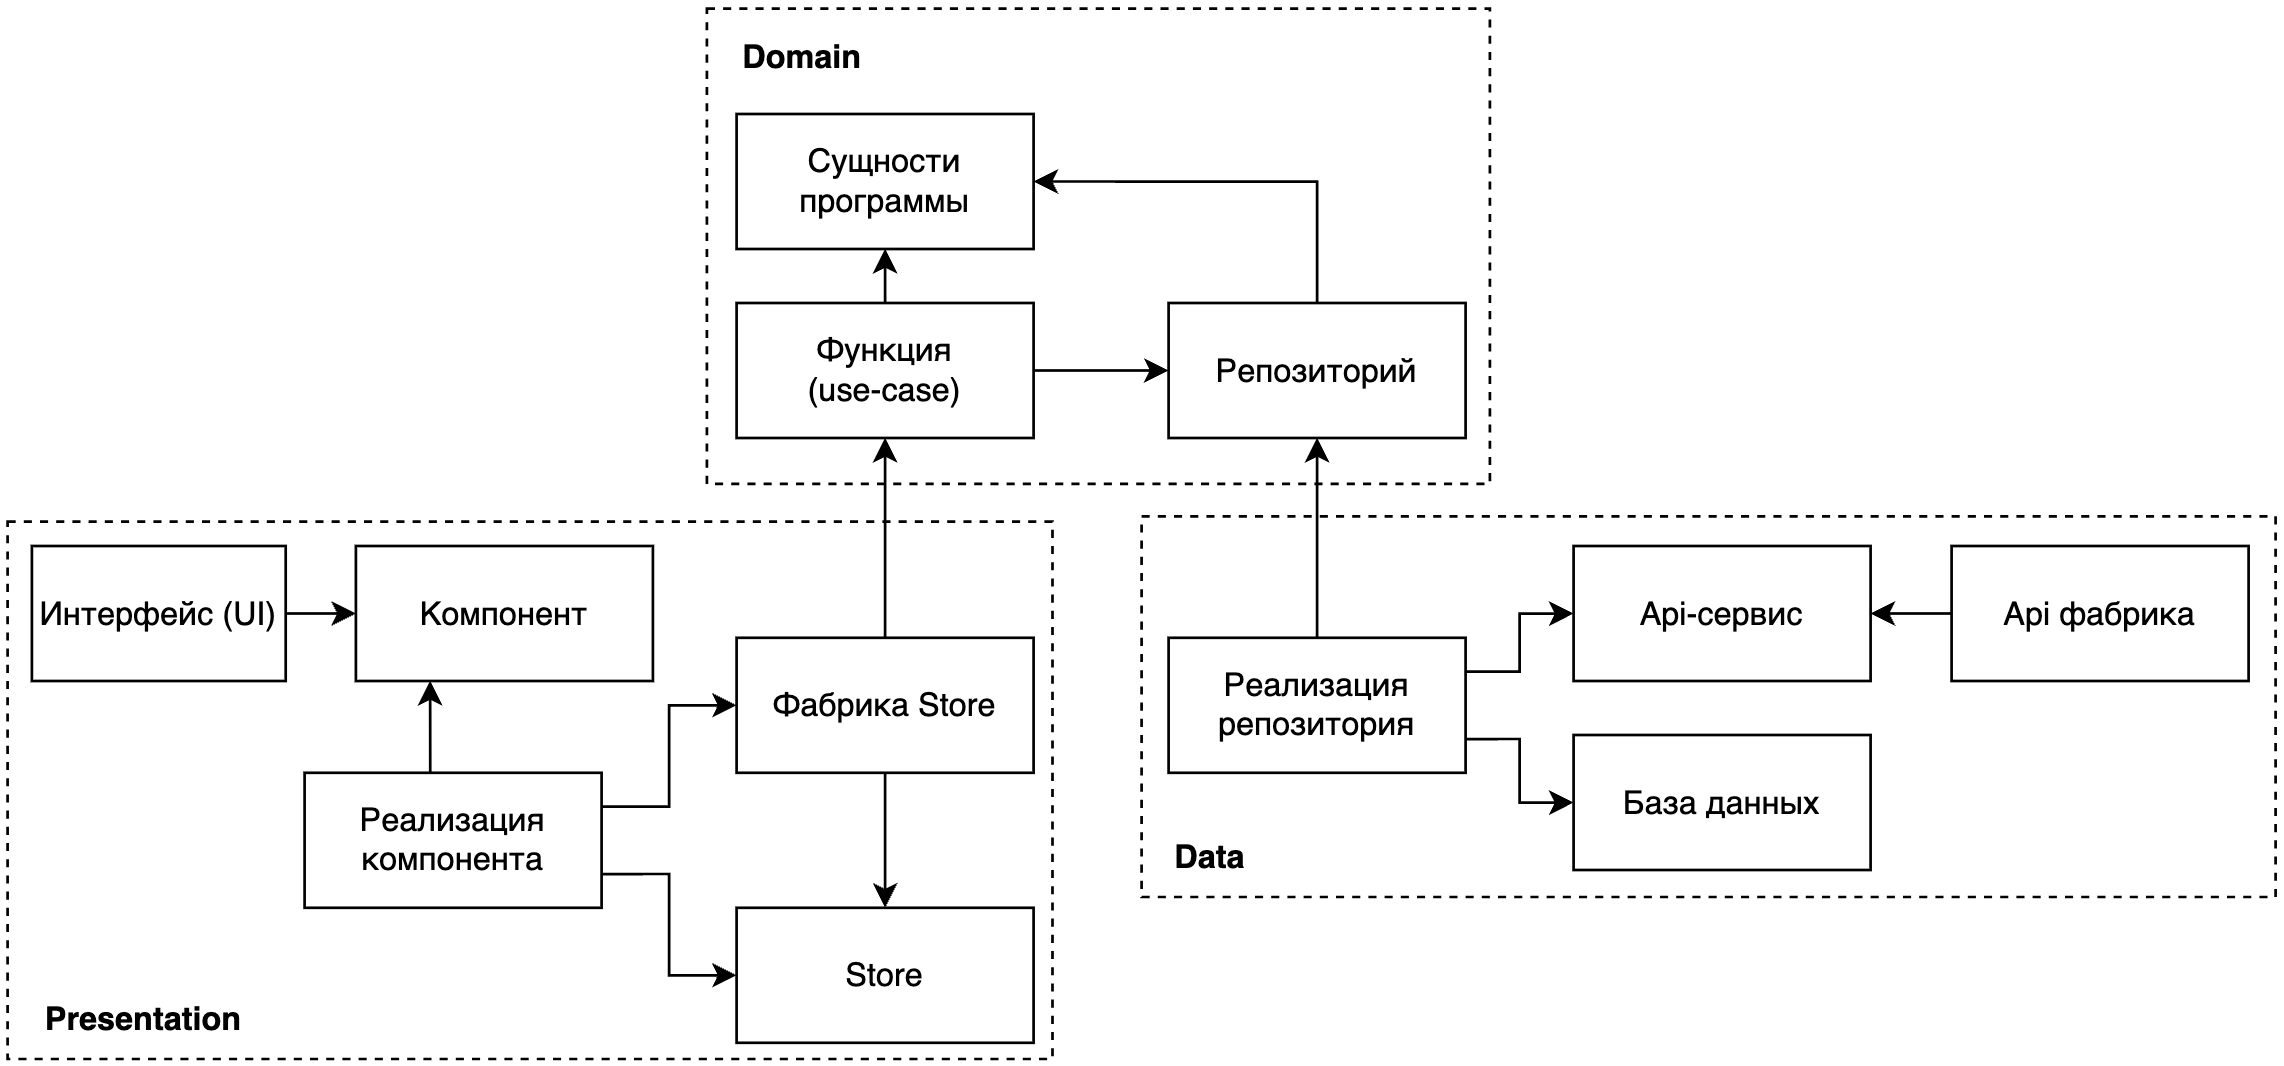
\includegraphics[height=0.3\textheight, width=\textwidth]{tools/img/component.png}
	\caption{
        Архитектура приложения, стрелки показывают направления зависимостей между компонентами
    }
	\label{fig:component}
\end{figure}

\section*{Выводы из конструкторской части}
В данном разделе были спроектированы сущности базы данных и способ их хранения и разработана ролевая модель.
Также спроектирована архитектура приложения, использующего базу данных.
Таким образом, получена достаточная информация для реализации базы данных.